\chapter{Modules and Visibility}

\section{Introduction: The Need for Organization}
When writing simple academic exercises, a single monolithic source file is often sufficient. However, as projects evolve into systems that solve real-world problems, complexity naturally grows. A file with thousands of lines becomes unwieldy: it is difficult to navigate, hard to understand, and almost impossible for multiple people to work on simultaneously. 

To manage this complexity, we must divide our code into logical, bite-sized components. This practice provides several core benefits:
\begin{itemize}
    \item \textbf{Maintainability:} Dividing code into smaller pieces makes it easier to comprehend, modify, and extend over time, reducing the risk of unintended side effects.
    \item \textbf{Encapsulation:} By hiding implementation details, we ensure that other parts of the program interact only with a well-defined public interface. Think of a car: you interact with the steering wheel and pedals, but the internal engine mechanics remain safely enclosed under the hood. You don't need to touch them to drive, and keeping them closed off prevents you from accidentally breaking the engine.
    \item \textbf{Safety at Compile Time:} Rust's visibility system allows the compiler to detect logical errors and API abuse during compilation, increasing the reliability of the software.
    \item \textbf{Reusable Libraries:} Structuring code into well-designed modules and crates allows us to reuse components across projects, reducing duplication.
\end{itemize}

Rust provides a powerful module system designed specifically to handle these software engineering challenges, allowing us to build scalable and robust applications.

\section{The Rust Project Structure: Packages and Crates}

To understand how Rust organizes code, we must define its hierarchical project structure, which consists of \textbf{Packages}, \textbf{Crates}, and \textbf{Modules}.

\begin{insightbox}{Packages vs. Crates}
A \textbf{Package} is the highest level of organization. It is a container managed by Cargo (defined by a \texttt{Cargo.toml} file) that groups together one or more Crates. 
A \textbf{Crate} is the fundamental unit of compilation and versioning in Rust. When you invoke \texttt{cargo build}, the compiler processes a crate to produce either an executable binary or a library. The process of combining these crates is called \textit{linking}, which can be \textit{static} (the executable includes a full copy of the library code) or \textit{dynamic} (external code is loaded at runtime via \texttt{.dll}, \texttt{.so}, or \texttt{.dylib} files).
\end{insightbox}

\begin{memoryblock}
\textbf{Memory and Process Separation with Libraries}\\
The professor emphasizes a crucial operating system concept regarding libraries: "The library, in total, does not allow me to have a variable divided between two processes. Two processes are and remain separate." Even if multiple executables load the same dynamic library, they do not share memory or variables. The operating system might share the \textit{read-only code pages} in physical memory to save RAM, but the data segments remain strictly private to each running process. 

Furthermore, regarding linking:
\begin{itemize}
    \item \textbf{Static Linking:} The linking is done directly in the compilation phase. The resulting executable is larger but self-contained and stable.
    \item \textbf{Dynamic Linking:} The linking phase only injects markers (or stubs) into the executable. When the program is launched, the OS locates the DLL/SO/DYLIB and maps it into the process's memory space. This makes the executable smaller, but relies on the library being present on the target machine.
\end{itemize}
\end{memoryblock}

By default, when you create a new project, Cargo provides a binary crate with the root file \texttt{src/main.rs}. The \texttt{main} function inside this file serves as the entry point for the executable. If you want to create a library crate---code meant to be shared and reused---the root file is \texttt{src/lib.rs}. 

\subsection{Building Multiple Executables}
A single package can contain multiple executable binaries. For instance, in a network application, you might want a \texttt{client}, a \texttt{server}, and a \texttt{tool} executable that all share the same underlying logic. By placing your shared logic in \texttt{src/lib.rs} and adding additional source files in a \texttt{src/bin/} directory, Cargo will automatically compile each file in \texttt{src/bin/} as a separate binary. All these executables share the same dependencies, have the same version, and are compiled together, making it easy to maintain related applications.

\subsection{Versioning}
Libraries and packages are versioned using Semantic Versioning (e.g., \texttt{1.2.5}), composed of three parts:
\begin{itemize}
    \item \textbf{Major}: Incremented for incompatible API changes. As the professor notes: "The Major changes when a main function of the program changes, breaking the compatibility with the past... using file scripts in the CSV format, after I'm supporting file scripts in Excel format... the same program no longer reads those old ones."
    \item \textbf{Minor}: Incremented for adding new functionality in a backward-compatible manner. "The minor instead changes when our program adds a feature. I read the CSV first, then I read the Excel. The CSV continues to read them, no problem."
    \item \textbf{Patch (Build)}: Incremented for backward-compatible bug fixes. "The structure of the program is the same. But I removed bugs... It's very normal to see high numbers."
\end{itemize}

\section{Defining Modules and Visibility}

While crates define the overarching structure, \textbf{Modules} (\texttt{mod}) allow us to organize code within a crate. Modules group related functions, structs, traits, and enums together. You can think of modules as folders within your crate's file system, and indeed, they often map directly to the actual file system directory structure.

\begin{insightbox}{The Folder Analogy}
The professor compares creating modules to organizing university files: "You already do it in part... you are often divided into polytechnic, course 1, course 2, exercise 1, exercise 2. You have divided your documents into smaller pieces... so that when you have to find things, you can get there. The same goes for the code. We want to divide the code into smaller pieces... and it makes it available to those who need it."
\end{insightbox}

See Figure \ref{fig:module_tree} for a conceptual representation of how modules branch out from the crate root.

\begin{figure}[h]
    \centering
    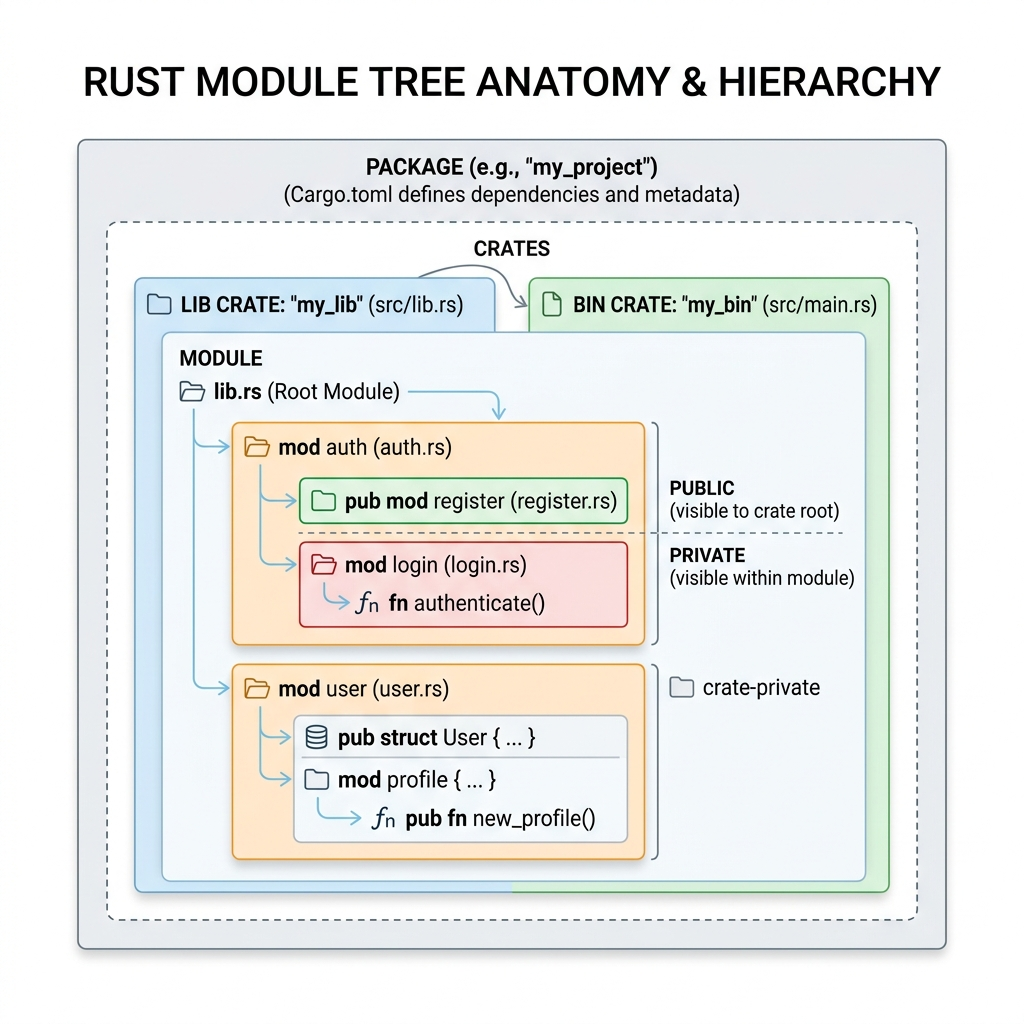
\includegraphics[width=0.7\textwidth]{images/module_tree.png}
    \caption{The hierarchical tree structure of modules originating from the crate root.}
    \label{fig:module_tree}
\end{figure}

\subsection{Modules and Source Files}
While modules can be declared inline, writing all code in a single file quickly defeats the purpose of modularity. Rust allows mapping modules to separate source files and directories:
\begin{itemize}
    \item \textbf{Inline Modules}: Declared within the same file using \texttt{mod name \{ ... \}}. Useful for small modules, such as isolating unit tests.
    \item \textbf{Separate Files}: A module named \texttt{my\_mod} can be placed in a file named \texttt{my\_mod.rs} in the same directory. The parent module simply declares it with \texttt{mod my\_mod;}. If this declaration is missing, the file is completely ignored by the compiler.
    \item \textbf{Directories for Sub-modules}: If \texttt{my\_mod} contains further sub-modules, you can create a folder named \texttt{my\_mod/} and place the sub-module files inside it. 
\end{itemize}

\begin{insightbox}{Inline Modules for Testing}
A common use case for inline modules is grouping tests. You can use the \texttt{\#[cfg(test)]} attribute on an inline module to tell the compiler to only include this code when running tests:
\begin{lstlisting}[language=Rust]
#[cfg(test)]
mod tests {
    use super::*; // Import symbols from the parent module

    #[test]
    fn test_hello() {
        // Test implementation here
    }
}
\end{lstlisting}
This keeps test code close to the implementation but prevents it from bloating the compiled release binary.
\end{insightbox}

\subsection{The \texttt{mod} and \texttt{pub} Keywords}

In Rust, all items (functions, structs, fields, modules) are \textbf{private by default}. They are only visible to the module in which they are defined and its descendants. To make an item accessible from outside its module, we use the \texttt{pub} keyword. This explicit visibility model is the cornerstone of encapsulation in Rust.

Let's look at an example demonstrating module declaration and visibility rules.

\begin{lstlisting}[language=Rust]
// src/lib.rs

// Declare a module named 'network'. 
// The compiler will look for its contents inline, in 'network.rs', or 'network/mod.rs'.
pub mod network {
    // A public struct
    pub struct ServerConfig {
        pub port: u16,       // Public field, accessible anywhere
        ip_address: String,  // Private field, only accessible within 'network'
    }

    impl ServerConfig {
        // A public constructor to instantiate the struct
        pub fn new(port: u16, ip: &str) -> Self {
            ServerConfig {
                port,
                ip_address: ip.to_string(),
            }
        }
    }

    // A private function, an internal implementation detail
    fn log_connection() {
        println!("New connection established.");
    }
}
\end{lstlisting}

\textbf{Practical Usage - When and Why to Use It:} Use this pattern when you want to enforce validation or initialization logic. By keeping fields private, you force clients to use the \texttt{new} constructor, preventing them from creating structurally invalid states (e.g., an invalid IP format) and controlling the instantiation process.

\textbf{Deep Memory Model Analysis:} In the constructor \texttt{pub fn new(port: u16, ip: \&str) -> Self}, the \texttt{port} parameter is passed by value. Because \texttt{u16} implements the \texttt{Copy} trait, it is copied directly on the stack into the new \texttt{ServerConfig} instance. The \texttt{ip} parameter is a string slice (\texttt{\&str}), which is a borrowed reference pointing to string data elsewhere (stack, heap, or static memory). However, the \texttt{ServerConfig} struct needs to own its data to be safely returned and dropped later. The call to \texttt{ip.to\_string()} performs a heap allocation, copying the character data into a newly allocated \texttt{String}. The ownership of this heap-allocated \texttt{String} is then transferred into the \texttt{ServerConfig} struct, giving it full ownership and a lifetime independent of the original \texttt{ip} slice.

In this snippet, \texttt{network} is a public module containing the \texttt{ServerConfig} struct. While the struct itself is public, its \texttt{ip\_address} field remains private. This means external code cannot directly instantiate \texttt{ServerConfig} using a struct literal because it cannot provide the private field; it must use the provided \texttt{pub fn new} constructor. This guarantees that internal invariants are maintained and users cannot bypass the intended logic.

\begin{notebox}
If a module is private, all of its contents are unreachable from the outside, even if those contents are marked with \texttt{pub}. The \texttt{pub} keyword only opens visibility up to the next level of the module hierarchy. A complete, uninterrupted chain of \texttt{pub} declarations is required to expose an item to the external API.
\end{notebox}

\subsection{Navigating Paths and Re-exporting}

To use an item from another module, we must specify its path. Paths can be \textit{absolute} or \textit{relative}:
\begin{itemize}
    \item \textbf{Absolute paths} start from the crate root using the \texttt{crate::} prefix (e.g., \texttt{crate::network::ServerConfig}) or an external crate name (e.g., \texttt{std::mem::size\_of\_val}).
    \item \textbf{Relative paths} start from the current module. They can start directly with a module identifier, or use \texttt{self::} (representing the current module, like \texttt{./} in a filesystem) and \texttt{super::} (representing the parent module, like \texttt{../} in a filesystem).
\end{itemize}

Typing long absolute paths is tedious. We can bring a path into the current scope using the \texttt{use} keyword, functioning like an alias.

\begin{insightbox}{The "Friend" Analogy for \texttt{use}}
The professor compares the \texttt{use} keyword to how we address people: "When you're dealing with a stranger, you call him Mario Rossi [full path]. When that's your friend, you call him Mario. \texttt{use} is simply saying this, which I know. So you don't have to give it all the genealogy."
\end{insightbox}

\begin{lstlisting}[language=Rust]
use crate::network::ServerConfig;

fn main() {
    let config = ServerConfig::new(8080, "127.0.0.1");
}
\end{lstlisting}

\begin{warningbox}
\textbf{Wildcard Imports (\texttt{*}):} You can use an asterisk to import all public items from a module (\texttt{use module::*;}). The professor warns against this: "It's not necessarily a great idea... because we carry on with things that we don't control. There could be someone of whom we don't know, whose name coincides with another of our names, and we get behaviors that we don't want." Always prefer explicit imports.
\end{warningbox}

Sometimes, a module's internal hierarchy is complex, but we want to provide a flat, simple API to the users of our library. We can achieve this using \textbf{re-exporting} with \texttt{pub use}. This takes an item defined in a deeply nested, possibly private module and exposes it at a higher level, effectively decoupling our internal code organization from the public interface we present to the world.

\begin{examprioritybox}{Re-exporting for API Stability (\texttt{pub use})}
The professor strongly emphasizes that designing for evolvability is the main reason to use modularity in real-world systems. Re-exporting is critical here: by exposing internals through a \texttt{pub use} facade in the library root, you can completely reorganize the internal sub-modules (e.g., switching from an old \texttt{beta} module to a \texttt{beta\_v2} module) without breaking the code of any user who depends on your library.

\textbf{Common Pitfall:} Exposing complex, deeply nested module structures to clients (e.g., forcing them to write \texttt{crate::internal::submodule::details::MyStruct}). This tightly couples the client to your internal structure, making future refactoring impossible without breaking changes.

\textbf{Expected Mastery Level:} High. You must know how to refactor internal modules while keeping the public API stable using \texttt{pub use}.
\end{examprioritybox}

\section{External Dependencies}

No system exists in isolation. Rust's package manager, Cargo, makes it incredibly easy to leverage the broader ecosystem of external crates hosted on \texttt{crates.io}. 

To add an external library, we declare it in the \texttt{[dependencies]} section of our \texttt{Cargo.toml} file. For example, to include \texttt{clap}, a popular declarative library for parsing command-line interfaces:

\begin{lstlisting}[language=toml]
[dependencies]
clap = { version = "4.5", features = ["derive"] }
\end{lstlisting}

When you next run \texttt{cargo build}, Cargo will automatically fetch, resolve, and compile the external library from \texttt{crates.io}. 

Using the \texttt{derive} feature, \texttt{clap} allows us to declaratively define our command-line arguments using a struct:

\begin{lstlisting}[language=Rust]
use clap::Parser;

#[derive(Parser, Debug)]
#[command(version, about = "A simple greeting program")]
struct Args {
    /// Name of the person to greet
    #[arg(short, long)]
    name: String,

    /// Number of times to greet
    #[arg(short, long, default_value_t = 1)]
    count: u8,
}

fn main() {
    let args = Args::parse();
    for _ in 0..args.count {
        println!("Hello {}!", args.name);
    }
}
\end{lstlisting}

\textbf{Practical Usage - When and Why to Use It:} Use declarative macro-based parsing (like \texttt{clap}'s \texttt{derive} feature) whenever building command-line utilities. It drastically reduces boilerplate error-handling and automatically provides help menus, bounds checking, and type conversion.

\textbf{Deep Memory Model Analysis:} The call to \texttt{Args::parse()} parses the environment arguments and constructs the \texttt{Args} struct. The \texttt{args.name} field is of type \texttt{String}, which means the parsed string argument has been copied into a new heap allocation, and the ownership of this heap memory is given to the \texttt{args} instance living on the \texttt{main} function's stack. As \texttt{args} owns the data, there are no complex lifetime constraints tying the struct to the raw OS string arguments. When \texttt{main} completes, the \texttt{args} struct is dropped, recursively triggering the drop of the heap-allocated \texttt{name} string.

This approach leverages the builder pattern behind the scenes, automatically generating the logic required to parse incoming arguments, apply constraints, and populate the \texttt{Args} struct.

\begin{exambox}{The Standard Library Prelude}
Notice that we never have to write \texttt{use std::vec::Vec;} or \texttt{use std::string::String;}. This is because Rust automatically imports a small set of highly ubiquitous standard library items into every module. This automatic import is known as the \textbf{prelude} (\texttt{std::prelude}).

When you use library functions, "you are exploiting pieces of Rust's standard library. Vector is inside the library called STD. File is inside the library called STD::IO." Even though they are built-in, they function as external modules that are automatically linked.
\end{exambox}

\section{Foreign Function Interface (FFI)}

Rust's strict guarantees of memory safety and zero-cost abstractions make it an excellent choice for system-level programming. However, we often need to integrate Rust code with other programming languages, such as C or Python. This interoperability is achieved through a Foreign Function Interface (FFI).

To allow other languages to call our Rust code, we must compile our library as a \textbf{dynamic library} compatible with C calling conventions. 

\subsection{Building a Dynamic C-Library}
Rust supports multiple crate types for libraries, defined via the \texttt{crate-type} key in \texttt{Cargo.toml}:
\begin{itemize}
    \item \texttt{rlib}: A static Rust library (the default).
    \item \texttt{dylib}: A dynamic Rust library.
    \item \texttt{cdylib}: A dynamic library conforming to the C Application Binary Interface (ABI), exportable to other languages.
    \item \texttt{staticlib}: A static library conforming to the C ABI.
\end{itemize}

To build a library compatible with other languages, we modify our \texttt{Cargo.toml} to specify the crate type as \texttt{cdylib}:

\begin{lstlisting}[language=toml]
[lib]
crate-type = ["cdylib"]
\end{lstlisting}

If no \texttt{crate-type} is specified, Cargo defaults to building an \texttt{rlib} (Rust static library), which is highly optimized but only usable by other Rust programs. Setting it to \texttt{cdylib} generates a dynamic library specifically formatted for C-interoperability (\texttt{.dll} on Windows, \texttt{.so} on Linux, and \texttt{.dylib} on macOS).

Next, we write the Rust function we wish to expose. We must apply two crucial modifiers:
\begin{enumerate}
    \item \texttt{extern "C"}: This tells the Rust compiler to use the C Application Binary Interface (ABI) for this function, ensuring the way arguments are passed and values are returned matches what C (and Python) expects.
    \item \texttt{\#[unsafe(no\_mangle)]} (or \texttt{\#[no\_mangle]} in older editions): By default, the Rust compiler alters (mangles) function names to include type information for linking purposes (e.g., renaming \texttt{add} to \texttt{add\_i32\_i32} to handle parameters). This attribute disables mangling, ensuring the exported function retains exactly the name we gave it. The professor notes: "It's unsafe because it could break things" since the compiler can no longer guarantee symbol uniqueness or type safety across boundaries.
\end{enumerate}

\begin{lstlisting}[language=Rust]
// src/lib.rs

#[unsafe(no_mangle)]
pub extern "C" fn add_numbers(a: i32, b: i32) -> i32 {
    a + b
}
\end{lstlisting}

\begin{examprioritybox}{FFI Modifiers: \texttt{extern "C"} and \texttt{no\_mangle}}
The professor explicitly highlights this mechanism to show how Rust can be embedded as a high-performance engine within Python or C ecosystems. 

\textbf{Common Pitfall:} Forgetting \texttt{\#[unsafe(no\_mangle)]}. If omitted, the Rust compiler renames the function to something mangled like \texttt{\_ZN7libname11add\_numbers17h...E}, making it impossible for the Python \texttt{ctypes} module to find it by the name \texttt{add\_numbers}. Furthermore, failing to use \texttt{extern "C"} means the function will use the Rust ABI, which may pass arguments in different registers than the C ABI expects, leading to crashes or garbage data.

\textbf{Expected Mastery Level:} Medium. You should conceptually understand why these modifiers are mandatory for interoperability across language boundaries.
\end{examprioritybox}

When compiled with \texttt{cargo build --release}, Cargo will produce a dynamic library file (\texttt{.dll} on Windows, \texttt{.so} on Linux, or \texttt{.dylib} on macOS). 

\subsection{Calling Rust from Python}
Other languages can now load this compiled dynamic library and invoke the \texttt{add\_numbers} function. Here is an example of how Python can utilize our Rust code using its standard \texttt{ctypes} module:

\begin{lstlisting}[language=Python]
import ctypes
import os

# Load the dynamic library compiled by Rust
# Note: The extension depends on the OS (.so, .dll, or .dylib)
lib_path = os.path.abspath("target/release/libpack1.dylib")
rust_lib = ctypes.CDLL(lib_path)

# Configure the argument and return types
# The professor notes: "I am instructing Python on the interface of my function."
rust_lib.add_numbers.argtypes = (ctypes.c_int32, ctypes.c_int32)
rust_lib.add_numbers.restype = ctypes.c_int32

# Call the Rust function natively!
result = rust_lib.add_numbers(10, 32)
print(f"Rust calculated: {result}") # Output: Rust calculated: 42
\end{lstlisting}

\begin{warningbox}
FFI intrinsically bypasses some of Rust's safety checks because the compiler cannot guarantee the behavior of the foreign code calling into or being called by Rust. Designing robust FFI boundaries requires careful attention to memory ownership, data representation, and thread safety.
\end{warningbox}

\section{Domande ed Esercizi da Esami Passati}

Nessuna domanda specifica da esami passati è stata mappata direttamente su questo capitolo.
